\documentclass[11pt]{article}

\usepackage[letterpaper,margin=0.75in]{geometry}
\usepackage{booktabs}
\usepackage{graphicx}
\usepackage{listings}
\usepackage{mathtools}

\setlength{\parindent}{1.4em}

\begin{document}

\lstset{
  language=Python,
  basicstyle=\small,          % print whole listing small
  keywordstyle=\bfseries,
  identifierstyle=,           % nothing happens
  commentstyle=,              % white comments
  stringstyle=\ttfamily,      % typewriter type for strings
  showstringspaces=false,     % no special string spaces
  numbers=left,
  numberstyle=\tiny,
  numbersep=5pt,
  frame=tb,
}

\title{Lab 3 Report}

\author{Dallin Christensen}

\date{March 29, 2014}

\maketitle

\section{Congestion Control}
Using my code from the previous lab (Reliable Transport), I was able to implement congestion control using TCP Tahoe with just a few modifications. Those modifications include the implementation of three new features: slow start, a slow start threshold, and AIMD (Additive Increase Multiplicative Decrease).

\subsection{Slow Start}
At the start of the connection and after any kind of loss event, the cwnd (congestion window) is set to 1 MSS. Every time the sender receives an ACK for new data, the cwnd is incremented by the number of new bytes of data acknowledged.
\paragraph{Set cwnd to 1 MSS at start of connection} \hspace{2mm}
\begin{lstlisting}
def send(self,data):
  self.send_buffer += data
  self.cwnd = self.mss
  self.send_if_possible()
\end{lstlisting}
\paragraph{Set cwnd to 1 MSS on loss event} \hspace{2mm}
\begin{lstlisting}
def loss_event(self):
  self.threshold = max(self.cwnd/2, self.mss)
  self.cwnd = self.mss
\end{lstlisting}

\subsection{Slow Start Threshold}
Slow start ends when the congestion window exceeds or equals the threshold. Per the project specifications, the initial threshold was set at 100000 bytes.

\subsection{AIMD}
\subsubsection{Additive Increase}
Additive increase, rather than slow start, is used to increase the size of the congestion window once the congestion window is larger than the threshold. Every time the sender receives an ACK for new data, the congestion window increases by MSS*b/cwnd, where MSS is the maximum segment size (1000 bytes) and b is the number of new bytes acknowledged. The threshold is also increased to the size of the new congestion window.
\subsubsection{Multiplicative Decrease}
When a loss event is detected (a timeout), the threshold is set to max(cwnd/2,MSS) and cwnd is set to 1 MSS. By only cutting the threshold in half and by using slow start, we prevent throughput from decreasing significantly when loss rates are low. However, if multiple loss rates occur in succession, the threshold will quickly drop to 1 MSS.
\paragraph{Decrease threshold on loss event} \hspace{2mm}
\begin{lstlisting}
def loss_event(self):
  self.threshold = max(self.cwnd/2, self.mss)
  self.cwnd = self.mss
\end{lstlisting}

\paragraph{Slow start and AIMD} \hspace{2mm}
\begin{lstlisting}
# the sender getting an ACK from the receiver
def handle_ack(self, packet):
  ...
  new_bytes = packet.ack_number - self.received_ack_number

  if self.cwnd >= self.threshold:
    # Additive Increase
    self.cwnd += (self.mss*new_bytes)/self.cwnd
    self.threshold = self.cwnd
  else:
    # Slow Start
    self.cwnd += new_bytes
\end{lstlisting}


\section{Experiments}
A simulator was used to set up a simple network consisting of two nodes and and one bidirectional link.
\begin{center}

\includegraphics{two-nodes-one-link.png}
\end{center}

\subsection{One Flow}
The link bandwidth was set to 10 Mbps, the propagation delay to 10 ms, and the queue size to 100000 bytes (or 100 packets). I transfered a 1 MB text file across the link. 

\subsubsection{One Flow - 0\% Loss}
Initially I tried this experiment with a 0\% loss rate. The congestion window size starts out at 1 MSS and increases exponentially (using slow start) until it reaches the threshold. Because the threshold (100000 bytes) is the same size as our file, slow start increases the congestion window size at a rate faster than the node sends packets, so no queue ever forms and there is no queueing delay.

Slow start is evidenced in the sequence plot created from the initial experiment. To start off, only one packet is sent. Once the ACK for that packet is received, the congestion window is doubled in size and two packets are sent. Once those two ACKs are received, four packets are sent, then eight, etc.

\paragraph{Sequence Plot} \hspace{2mm}
\begin{center}
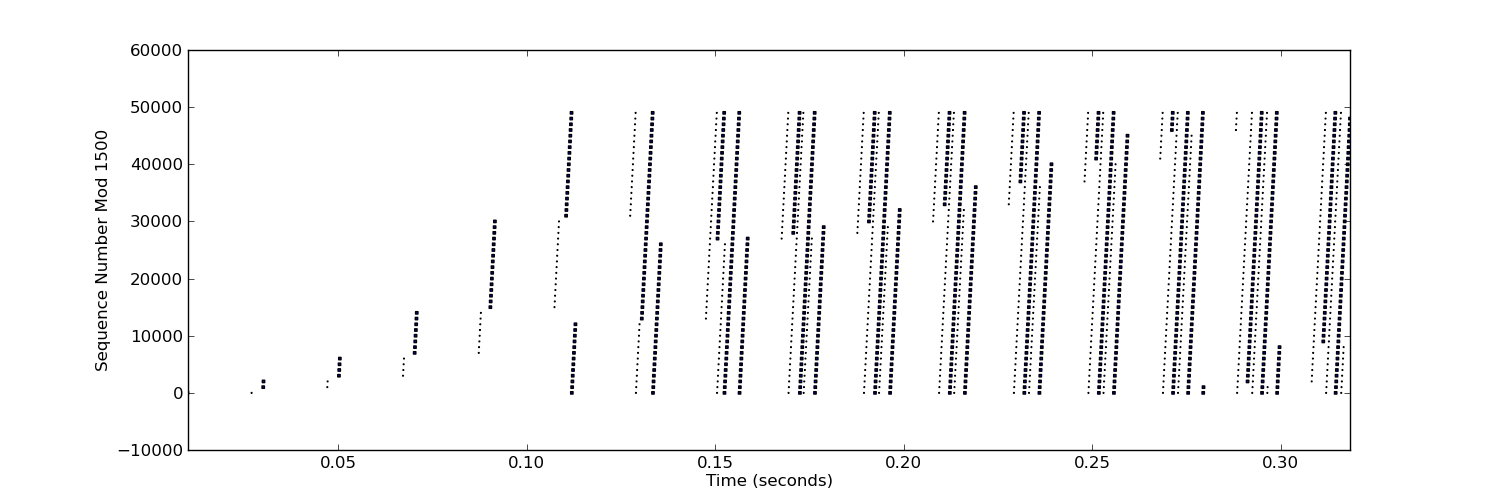
\includegraphics[width=20cm]{../plot/one_flow_0_loss/sequence.png}
\end{center}

Slow start is also evidenced in the window size plot. The congestion window doubles in size until it reaches the threshold (100 MSS), then increases additively after that. Had there been a loss rate, we would expect a sawtooth pattern, showing that the congestion window gets cut in half with every loss. But because this experiment had a 0\% loss rate, that sawtooth pattern is not shown.

\paragraph{Window Size Plot} \hspace{2mm}
\begin{center}
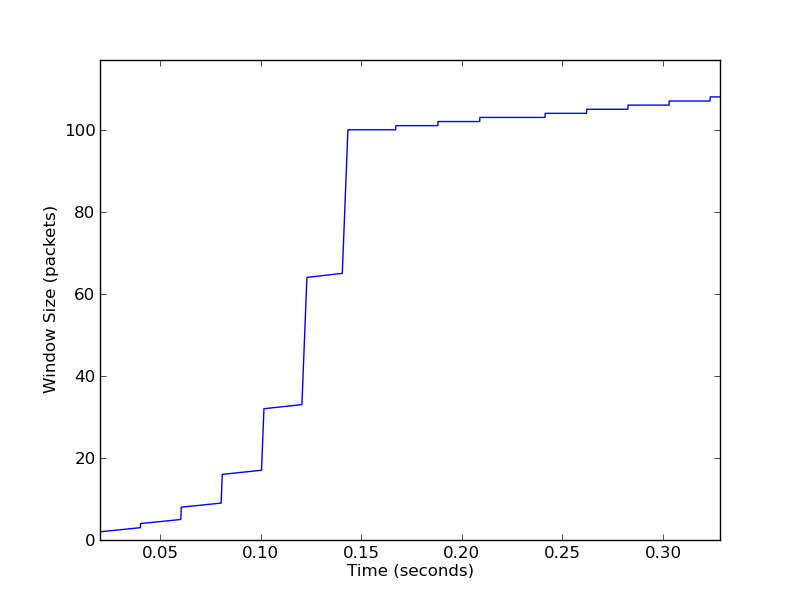
\includegraphics[width=15cm]{../plot/one_flow_0_loss/window_size.png}
\end{center}

The rate plot is clearly wrong, but I can't figure out why. I expected the rate to increase quickly until it reached the 10 Mbps bandwidth of the link, platueing there until the file finished transfering. However, when the experiment was run, the rate continued well beyond the 10 Mbps bandwidth and never platued.

\paragraph{Rate Plot} \hspace{2mm}
\begin{center}
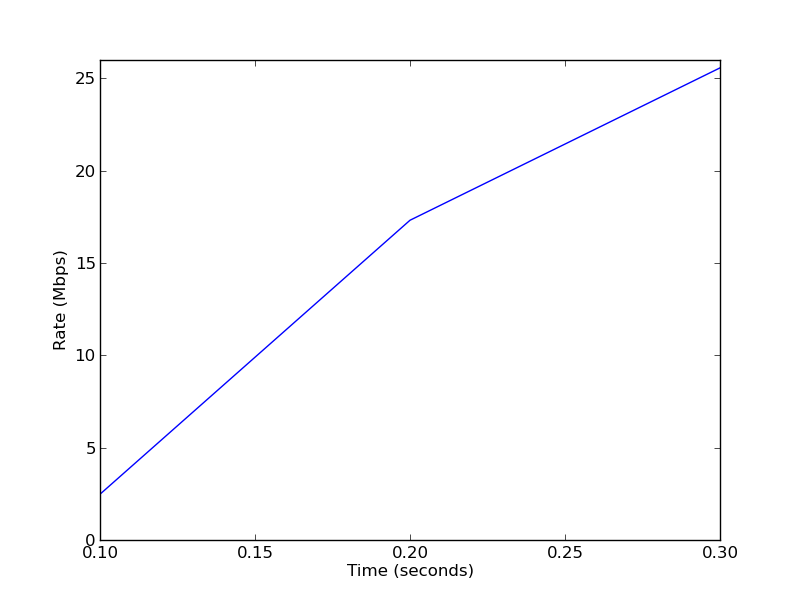
\includegraphics[width=15cm]{../plot/one_flow_0_loss/rate.png}
\end{center}

\subsubsection{One Flow - 1\% Loss}
The experiment was run again, but with a 1\% loss rate.

Loss events are noticeable on the sequence plot by the 0.1 second timeout that triggers a retransmission. Slow start is visible at the beginning of the connection, but does not seem to occur after retransmission events. This seems to contradict the code, but it was the observed behavior.

\paragraph{Sequence Plot} \hspace{2mm}
\begin{center}
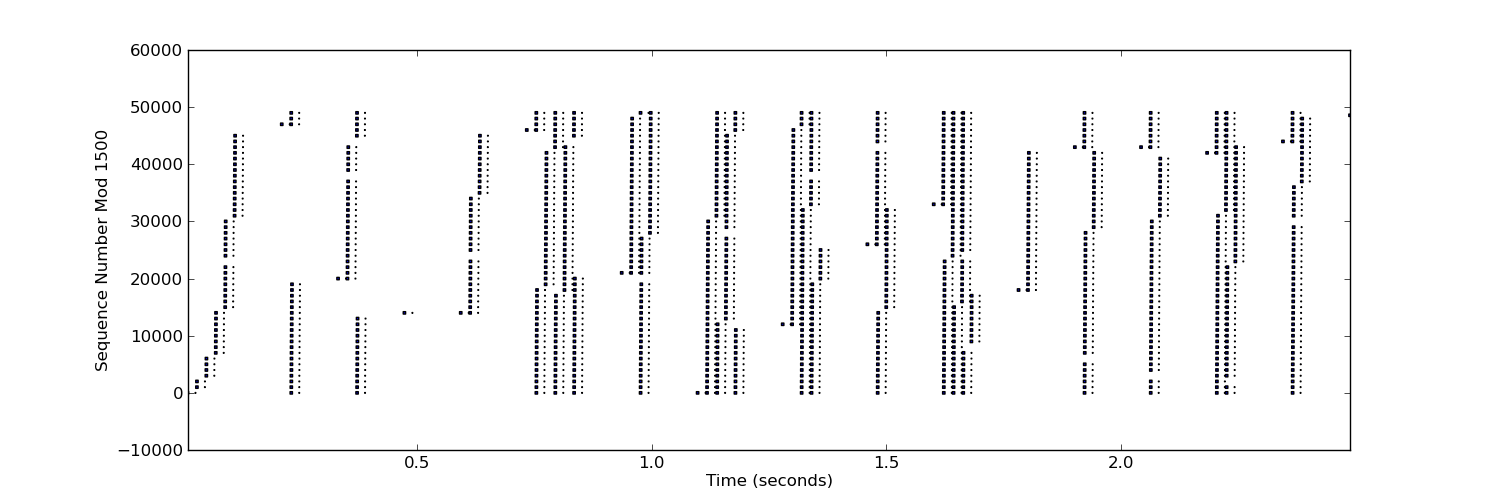
\includegraphics[width=20cm]{../plot/one_flow_1_loss/sequence.png}
\end{center}

The expected sawtooth pattern is visible in the window size plot. The congestion window gets cut down to 1 MSS with each loss event, and the window size never gets larger than the initial threshold as it did with a 0\% loss rate. The largest it ever got was about 45 packets.

\paragraph{Window Size Plot} \hspace{2mm}
\begin{center}
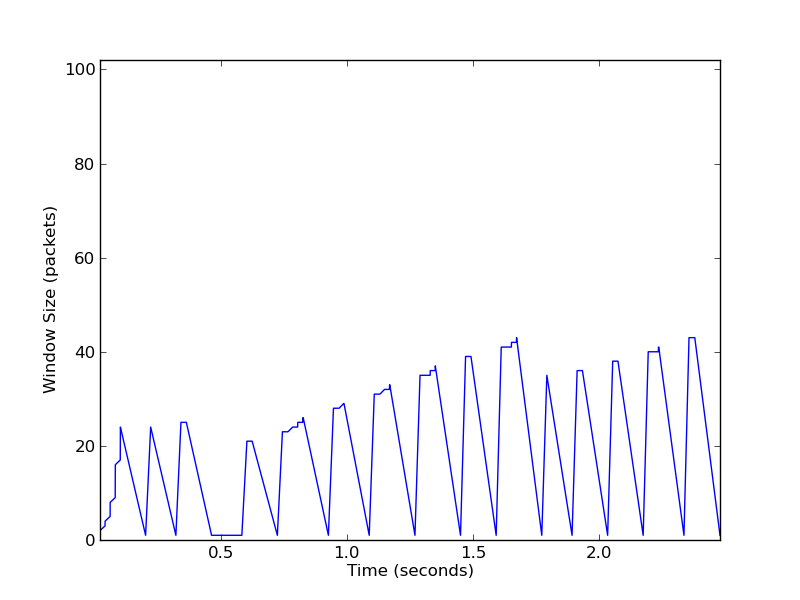
\includegraphics[width=15cm]{../plot/one_flow_1_loss/window_size.png}
\end{center}

When the experiment was rerun with a 1\% loss rate, the rate was a much more reasonable speed (~5 Mbps at it's peak) than the initial experiment.

\paragraph{Rate Plot} \hspace{2mm}
\begin{center}
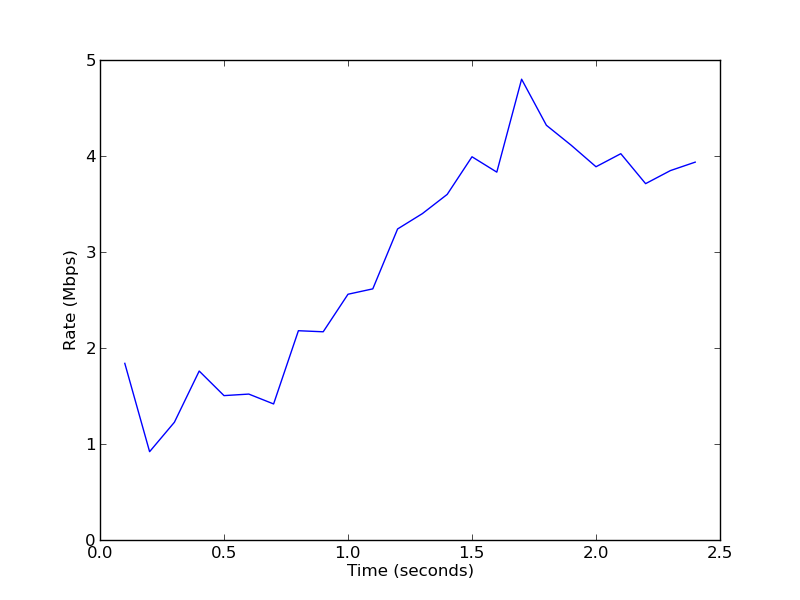
\includegraphics[width=15cm]{../plot/one_flow_1_loss/rate.png}
\end{center}

The loss events are noted on the queue plot, which is not included in this report, but can be viewed in the attached source files.

\subsubsection{One Flow - 5\% Loss}
The experiment was run again with a 5\% loss rate. As expected, loss events occur more frequently than they did in the previous experiments, occuring in a lower rate and smaller congestion window. These observances can be seen in the graphs included with the attached source files.

\subsection{Two Flows}
I repeated the same experiment, but with two TCP flows (using different ports). Each flow transferred the same 1 MB text file and they started at the same time. Unfortunately, I was unable to get the proper expected behavior when using two flows, even after countless attempts and many frustrating hours.
\subsection{Five Flows}
I also repeated the experiment with five TCP flows (using different ports). The flows had a staggered start, each one starting 0.1 seconds after the previous one. Unfortunately, as with the two flows, I was unable to get the proper expected behavior when using five flows, even after countless attempts and many frustrating hours.

\vspace{0.5cm}
\end{document}
